\documentclass[a4paper, 12pt]{article}
\usepackage{fancyhdr}
\usepackage[12pt]{moresize}
\usepackage[pdftex]{graphicx}
\usepackage{epstopdf}
\pagestyle{empty}
\addtolength{\oddsidemargin}{-.875in}
\addtolength{\evensidemargin}{-.875in}
\addtolength{\textwidth}{2in}
\addtolength{\topmargin}{-.2in}
\addtolength{\textheight}{2in}
\begin{document}
\begin{center}
	{\LARGE {\textbf {MM2090 ASSIGNMENT-4}}}
\end{center}

\section{Student Details}
\textbf {Name} : \textbf{\textit {Prithviraj Pratap Bhosle}}\\
\textbf {Roll No.} : \textbf{\textit {MM20B049}}\\
\textbf {Group} : \textbf{\textit {Group-7}}
\section{Change in Internal Energy of an Ideal Gas}
\subsection{Equation}
\begin{equation}
	{\LARGE{\textbf{$ \Delta U=n C_{v}  \Delta T $}}}
	\label{eq:1}
\end{equation}

{\normalsize { Here in equation \ref{eq:1}\\
{\normalsize {\textbf{$ \Delta U $} represents the the change in internal energy in an ideal gas}}\\
{\normalsize {\textbf{$ n $} \  represents the number of moles of the ideal gas}}\\
{\normalsize {\textbf{$ C_{v} $} \  represents the molar specific heat at constant volume of the ideal gas}}\\
{\normalsize {\textbf{$ \Delta T $} \  represents the change in temperature of the ideal gas}}
\subsection{Description}

{\small {Thermodynamics often uses the concept of the ideal gas for teaching purposes, and as an approximation for working systems. The ideal gas is a gas of particles considered as point objects that interact only by elastic collisions and fill a volume such that their mean free path between collisions is much larger than their diameter.\cite{IE} Such systems approximate the monatomic gases, helium and the other noble gases. Here the kinetic energy consists only of the translational energy of the individual atoms. Monatomic particles do not rotate or vibrate, and are not electronically excited to higher energies except at very high temperatures.

Therefore, internal energy changes in an ideal gas may be described solely by changes in its kinetic energy. Kinetic energy is simply the internal energy of the perfect gas and depends entirely on its pressure, volume and thermodynamic temperature.

The internal energy of an ideal gas is proportional to its number of moles n and to its temperature T. The temperature dependence of the change in internal energy of the ideal gas is plotted in the below graph (see figure \ref{fig:1}) \cite{Image}
\begin{figure}[h]
	\centerline{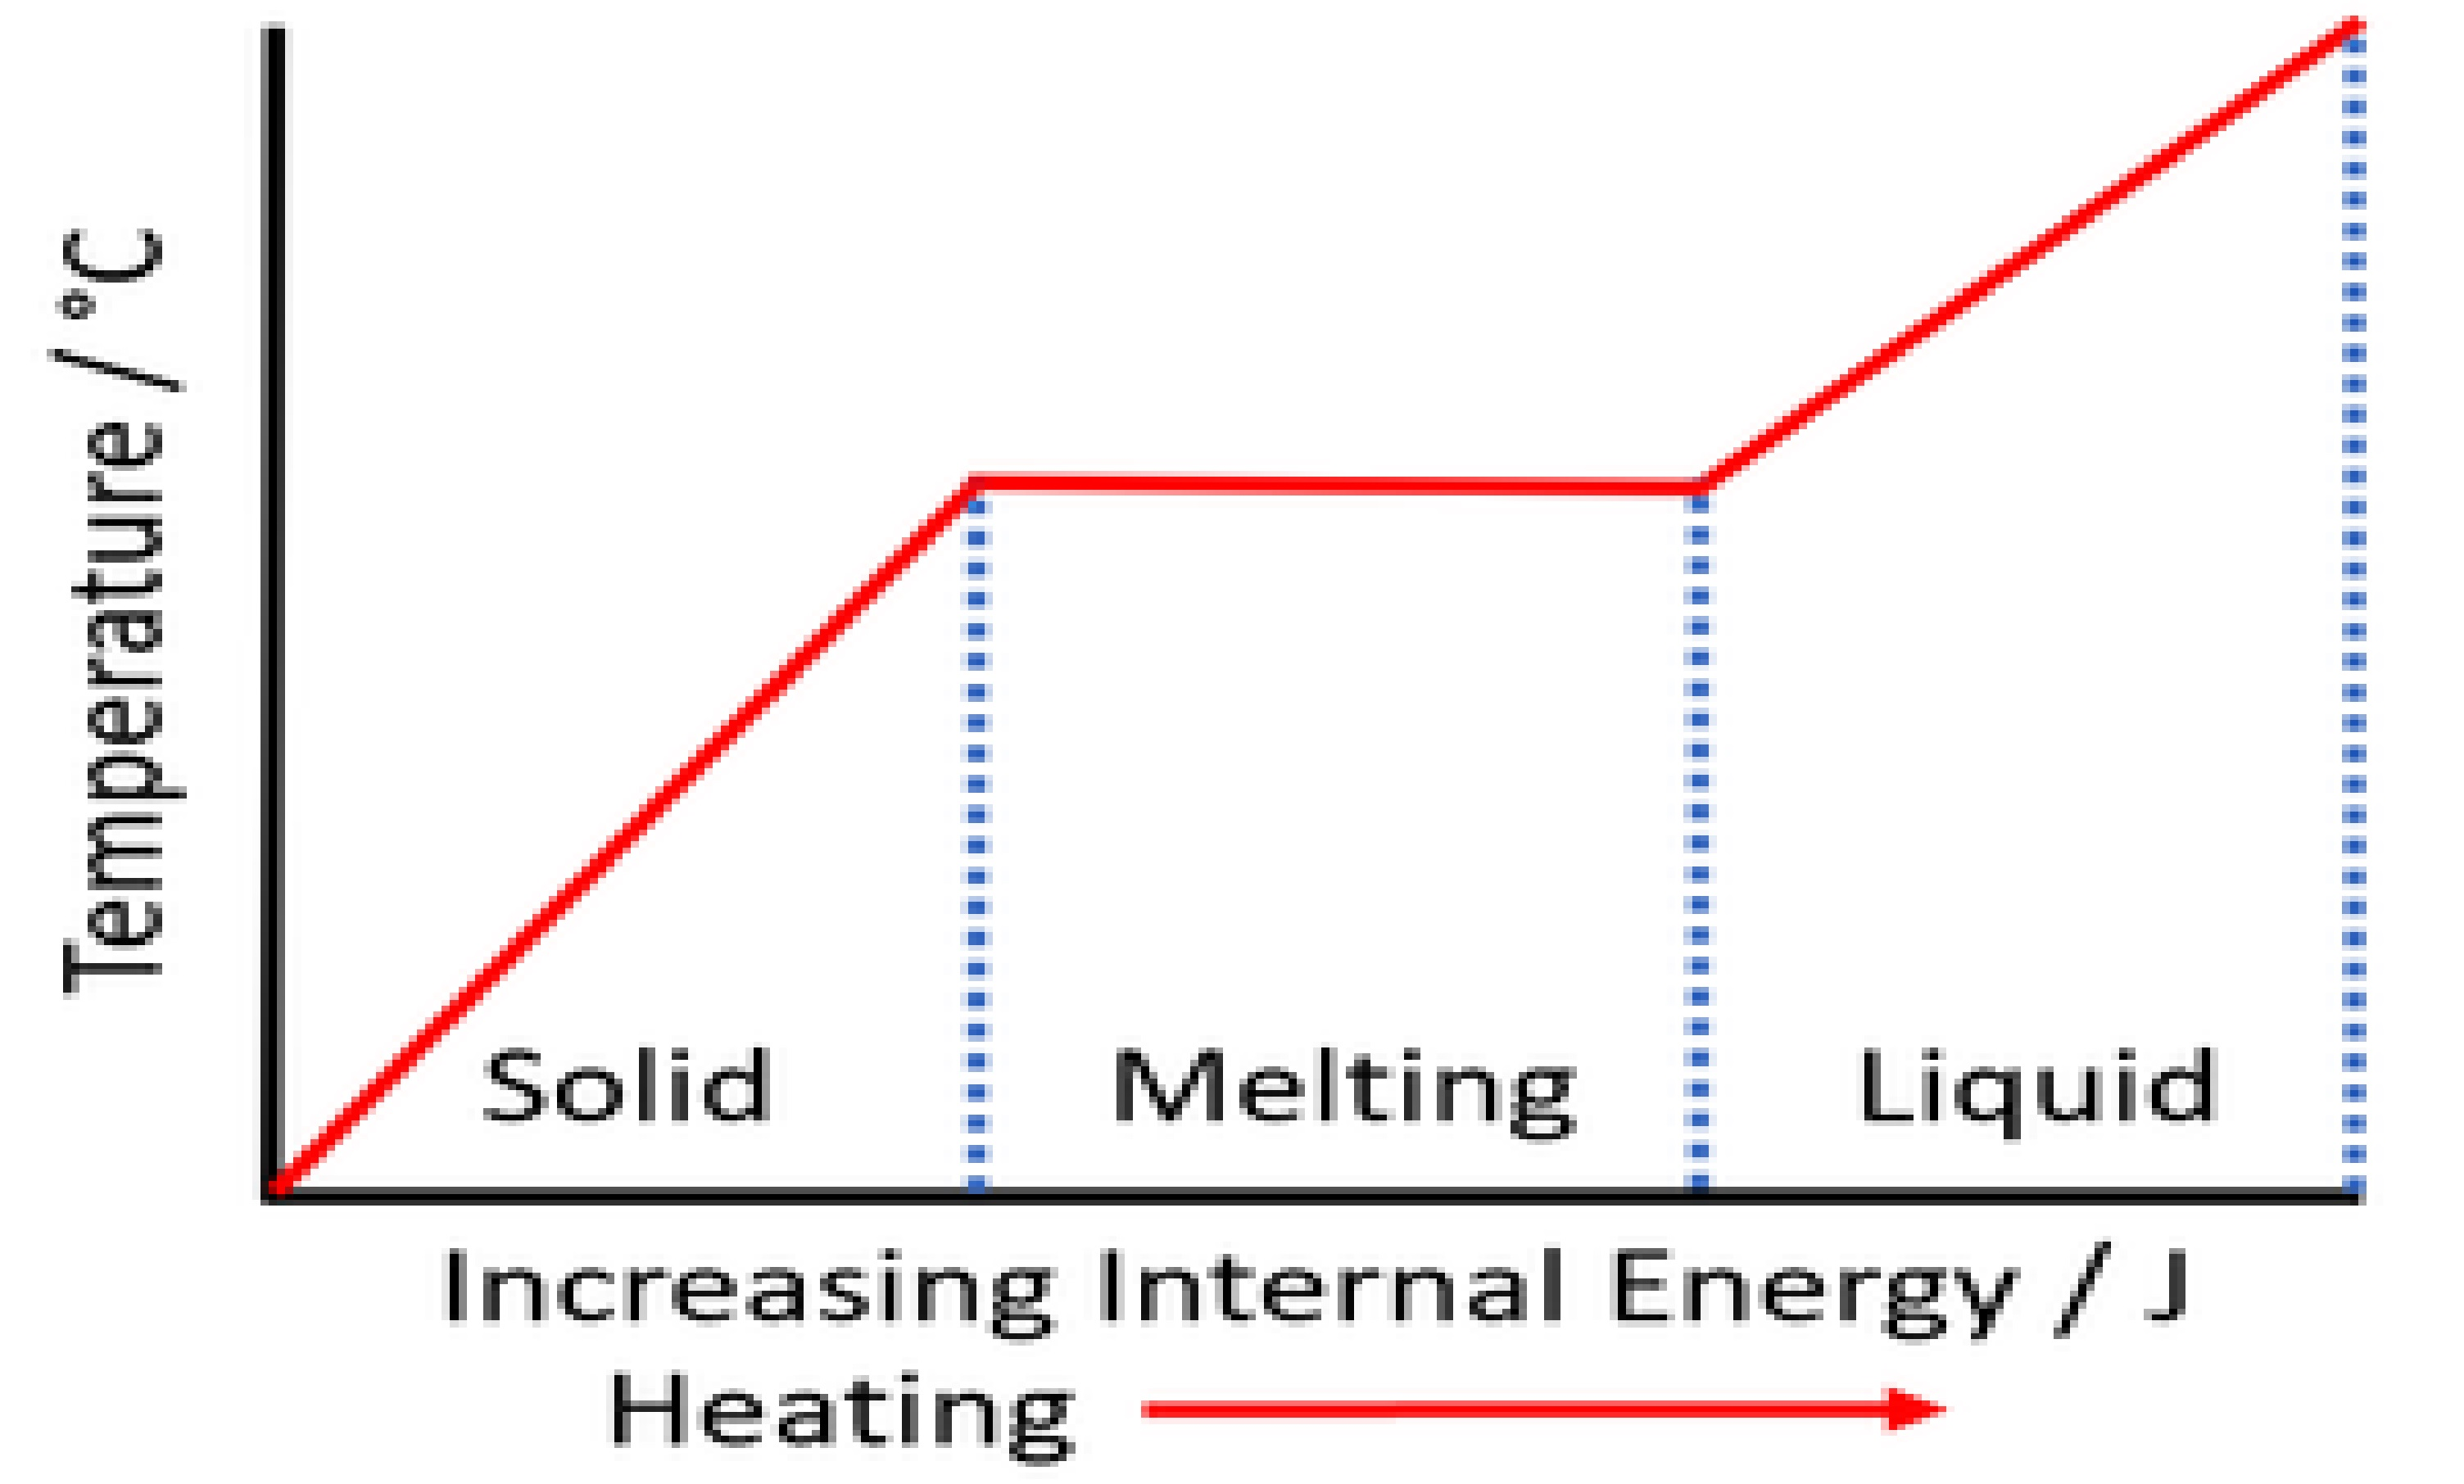
\includegraphics[scale=0.1]{MM20B049}}
	\caption{Internal Energy v/s Temperature graph}
        \label{fig:1}
\end{figure}

}}
\newpage
\bibliographystyle{plain}
\bibliography{mm20b049.bib}

\end{document}

